
\subsection{Single-version} \label{single}

Single-version is a category of techniques which focus on creating a singular, robust implementation of software by integrating safety checks and redundancies directly into the software design process \cite{nasa:sft}.

This technique emphasizes the detection of errors within the software and the ability to recover from them. Error detection typically involves monitoring the system for unexpected behaviors or inconsistencies, which could signal the presence of a fault \cite{shubu}. Recovery mechanisms then act to mitigate the effects of these faults.

Handling an error can be done in various ways. Most common would be to backtrack to a saved checkpoint and retry the part of the application where an error was discovered in the hopes of getting the correct result on the subsequent retries. This usually works well with transient faults, but it is likely to fail in the presence of a permanent fault.

Drawbacks of single version techniques are primarily the lack of alternatives and fallbacks, should the program fail. Single-version techniques heavily rely on error detection and recovery, which might not always work in practice. The reason single-version techniques are viable is an observation that transient faults are way more common than permanent faults \cite{1676899}, meaning that single-version is usually enough for noncritical parts of the system.

\subsubsection{Modularity}

Perhaps the simplest way we can create a more resilient software is to structure it into independent modules. Each module should handle one task and, when possible, not directly rely upon any other modules for its functionality.

A technique commonly utilized to achieve modularity is partitioning, which can be divided into horizontal and vertical partitioning. Horizontal partitioning aims to split the software into independent structural branches communicating through interfaces. 
Vertical partitioning splits the software in a top-down fashion, where higher level modules are tasked with control logic, while lower level modules do most of the processing \cite{nasa:sft}.

% \begin{figure}[!h]
% \centering
% \begin{minipage}{.6\textwidth}
%     \centering
%     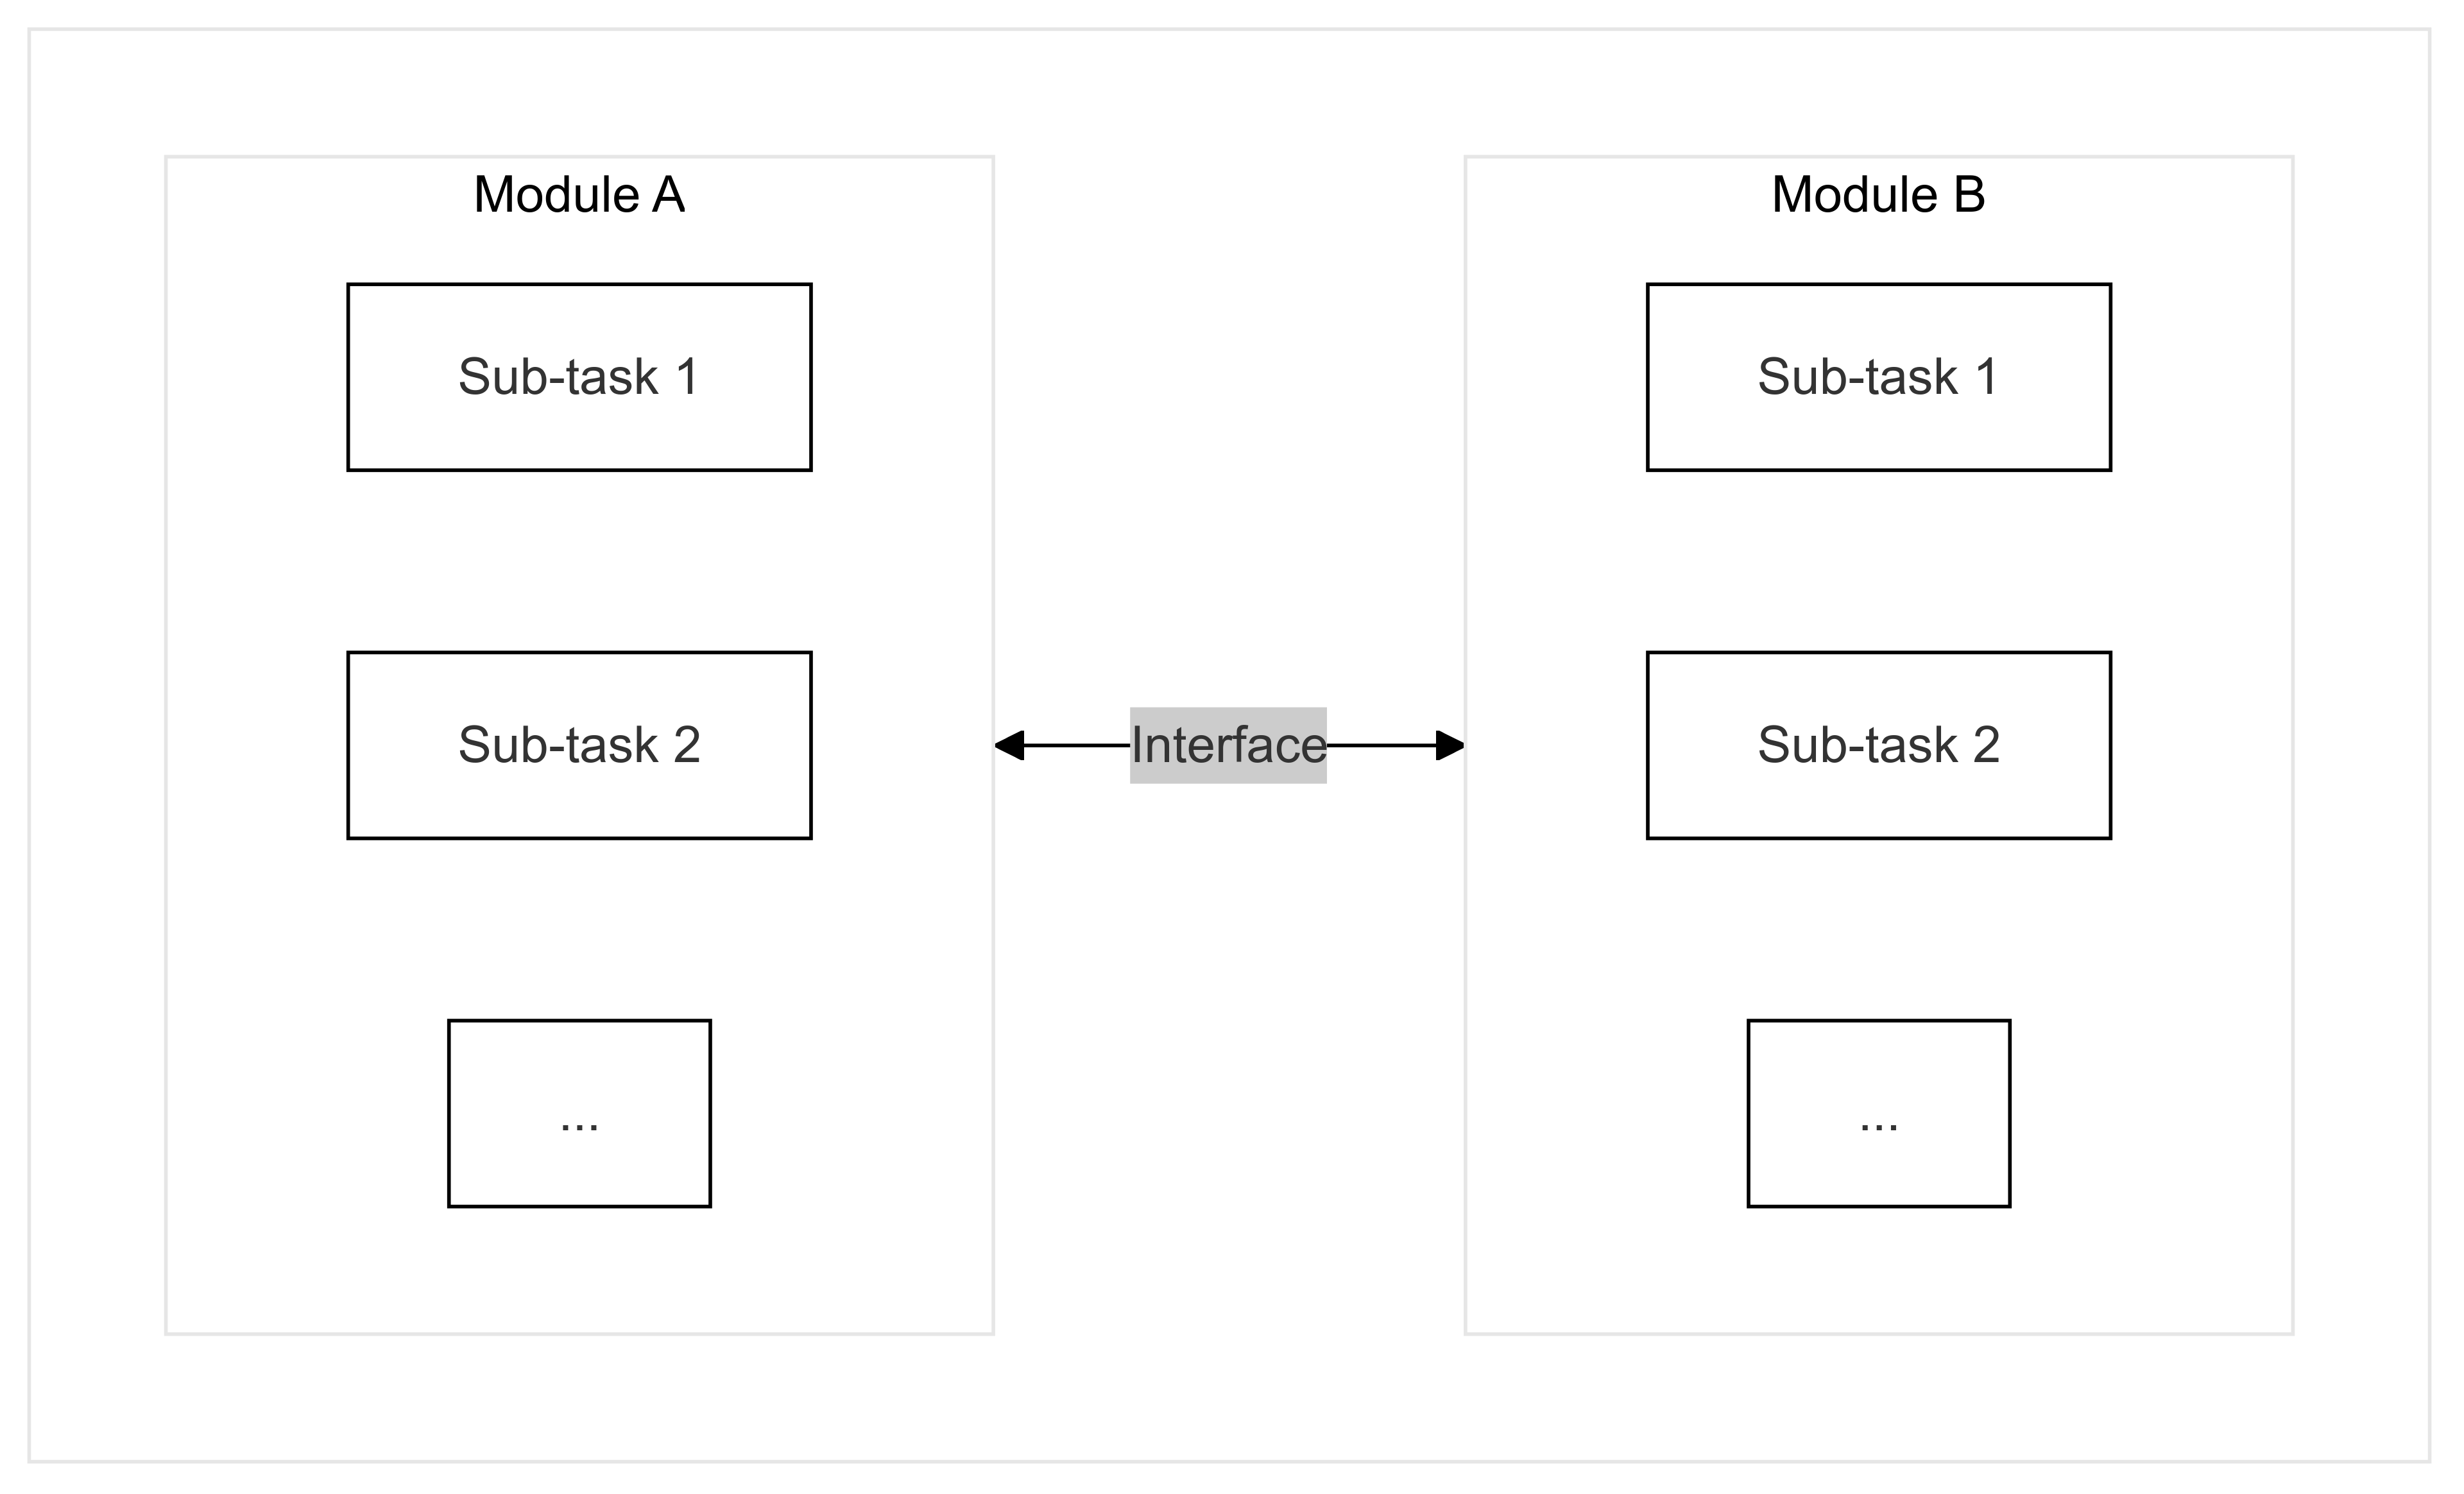
\includegraphics[width=0.7\textwidth]{modularity/horizontal.png}
%     \label{fig:mod_hor}
% \end{minipage}%
% \begin{minipage}{.6\textwidth}
%     \centering
%     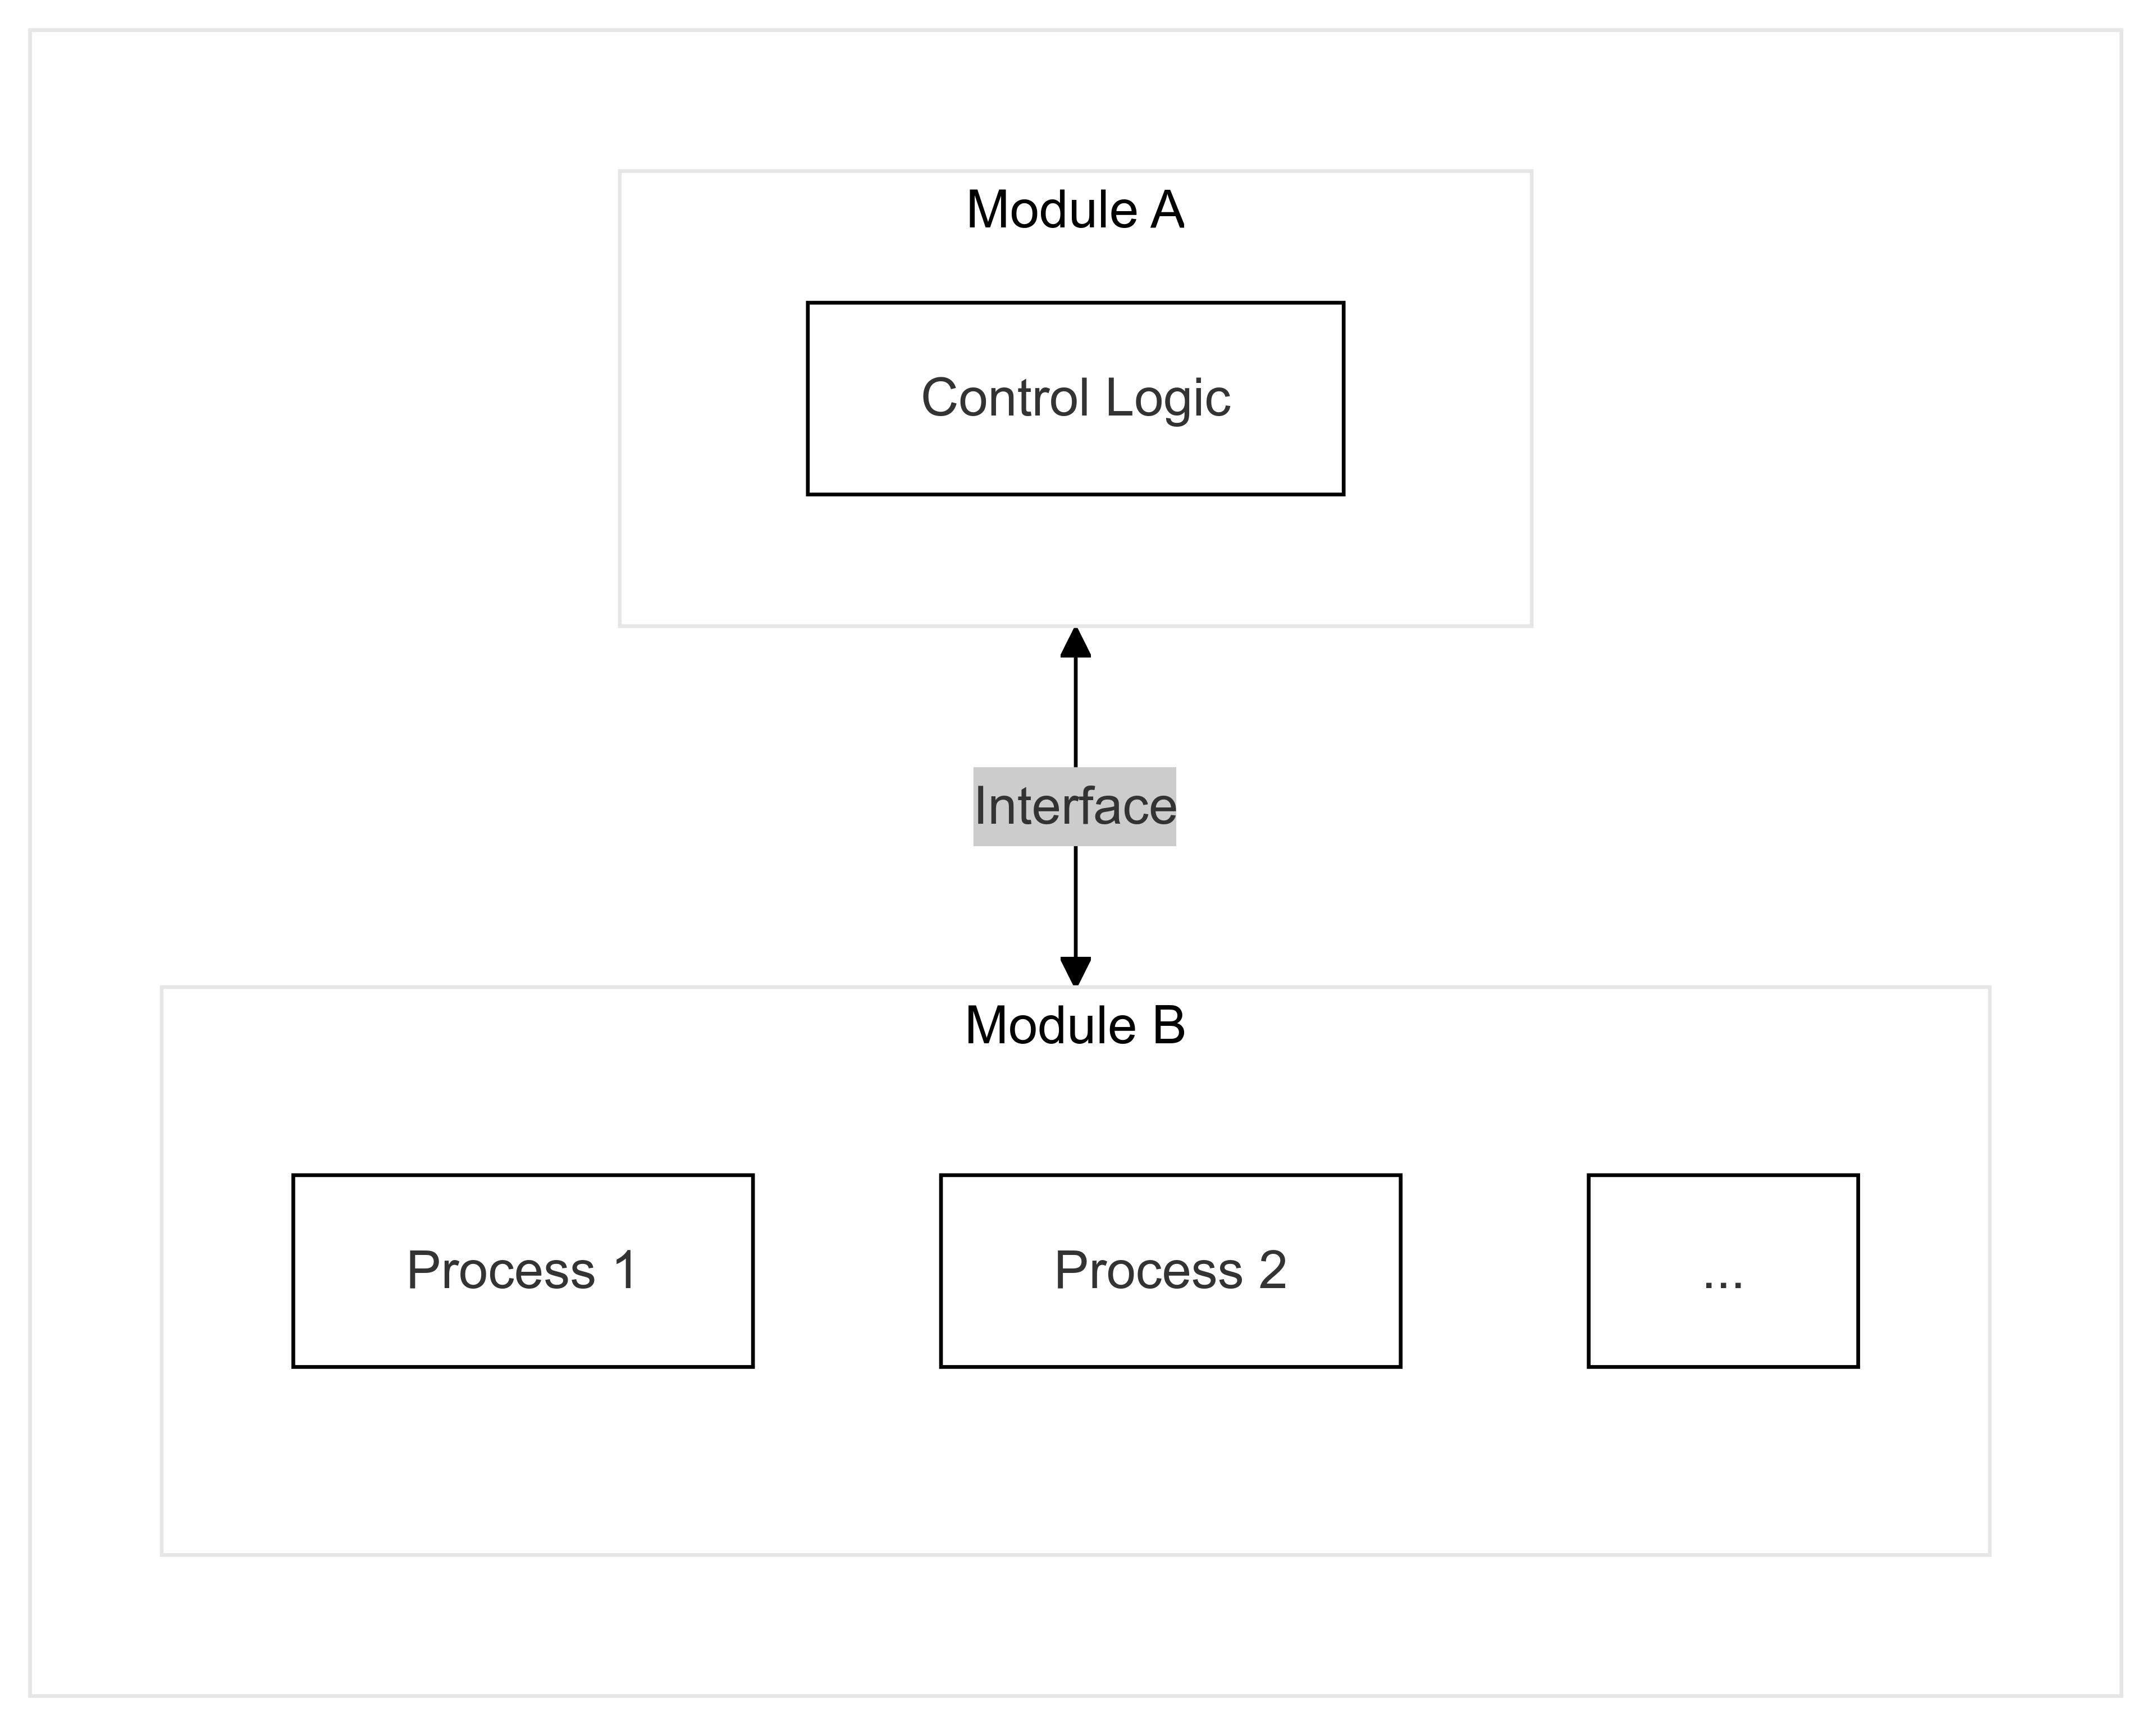
\includegraphics[width=0.7\textwidth]{modularity/vertical.png}
%     \label{fig:mod_ver}
% \end{minipage}
% \caption{Horizontal and vertical partitioning}
% \end{figure}

% \begin{figure}[hbt!]
%     \centering
%     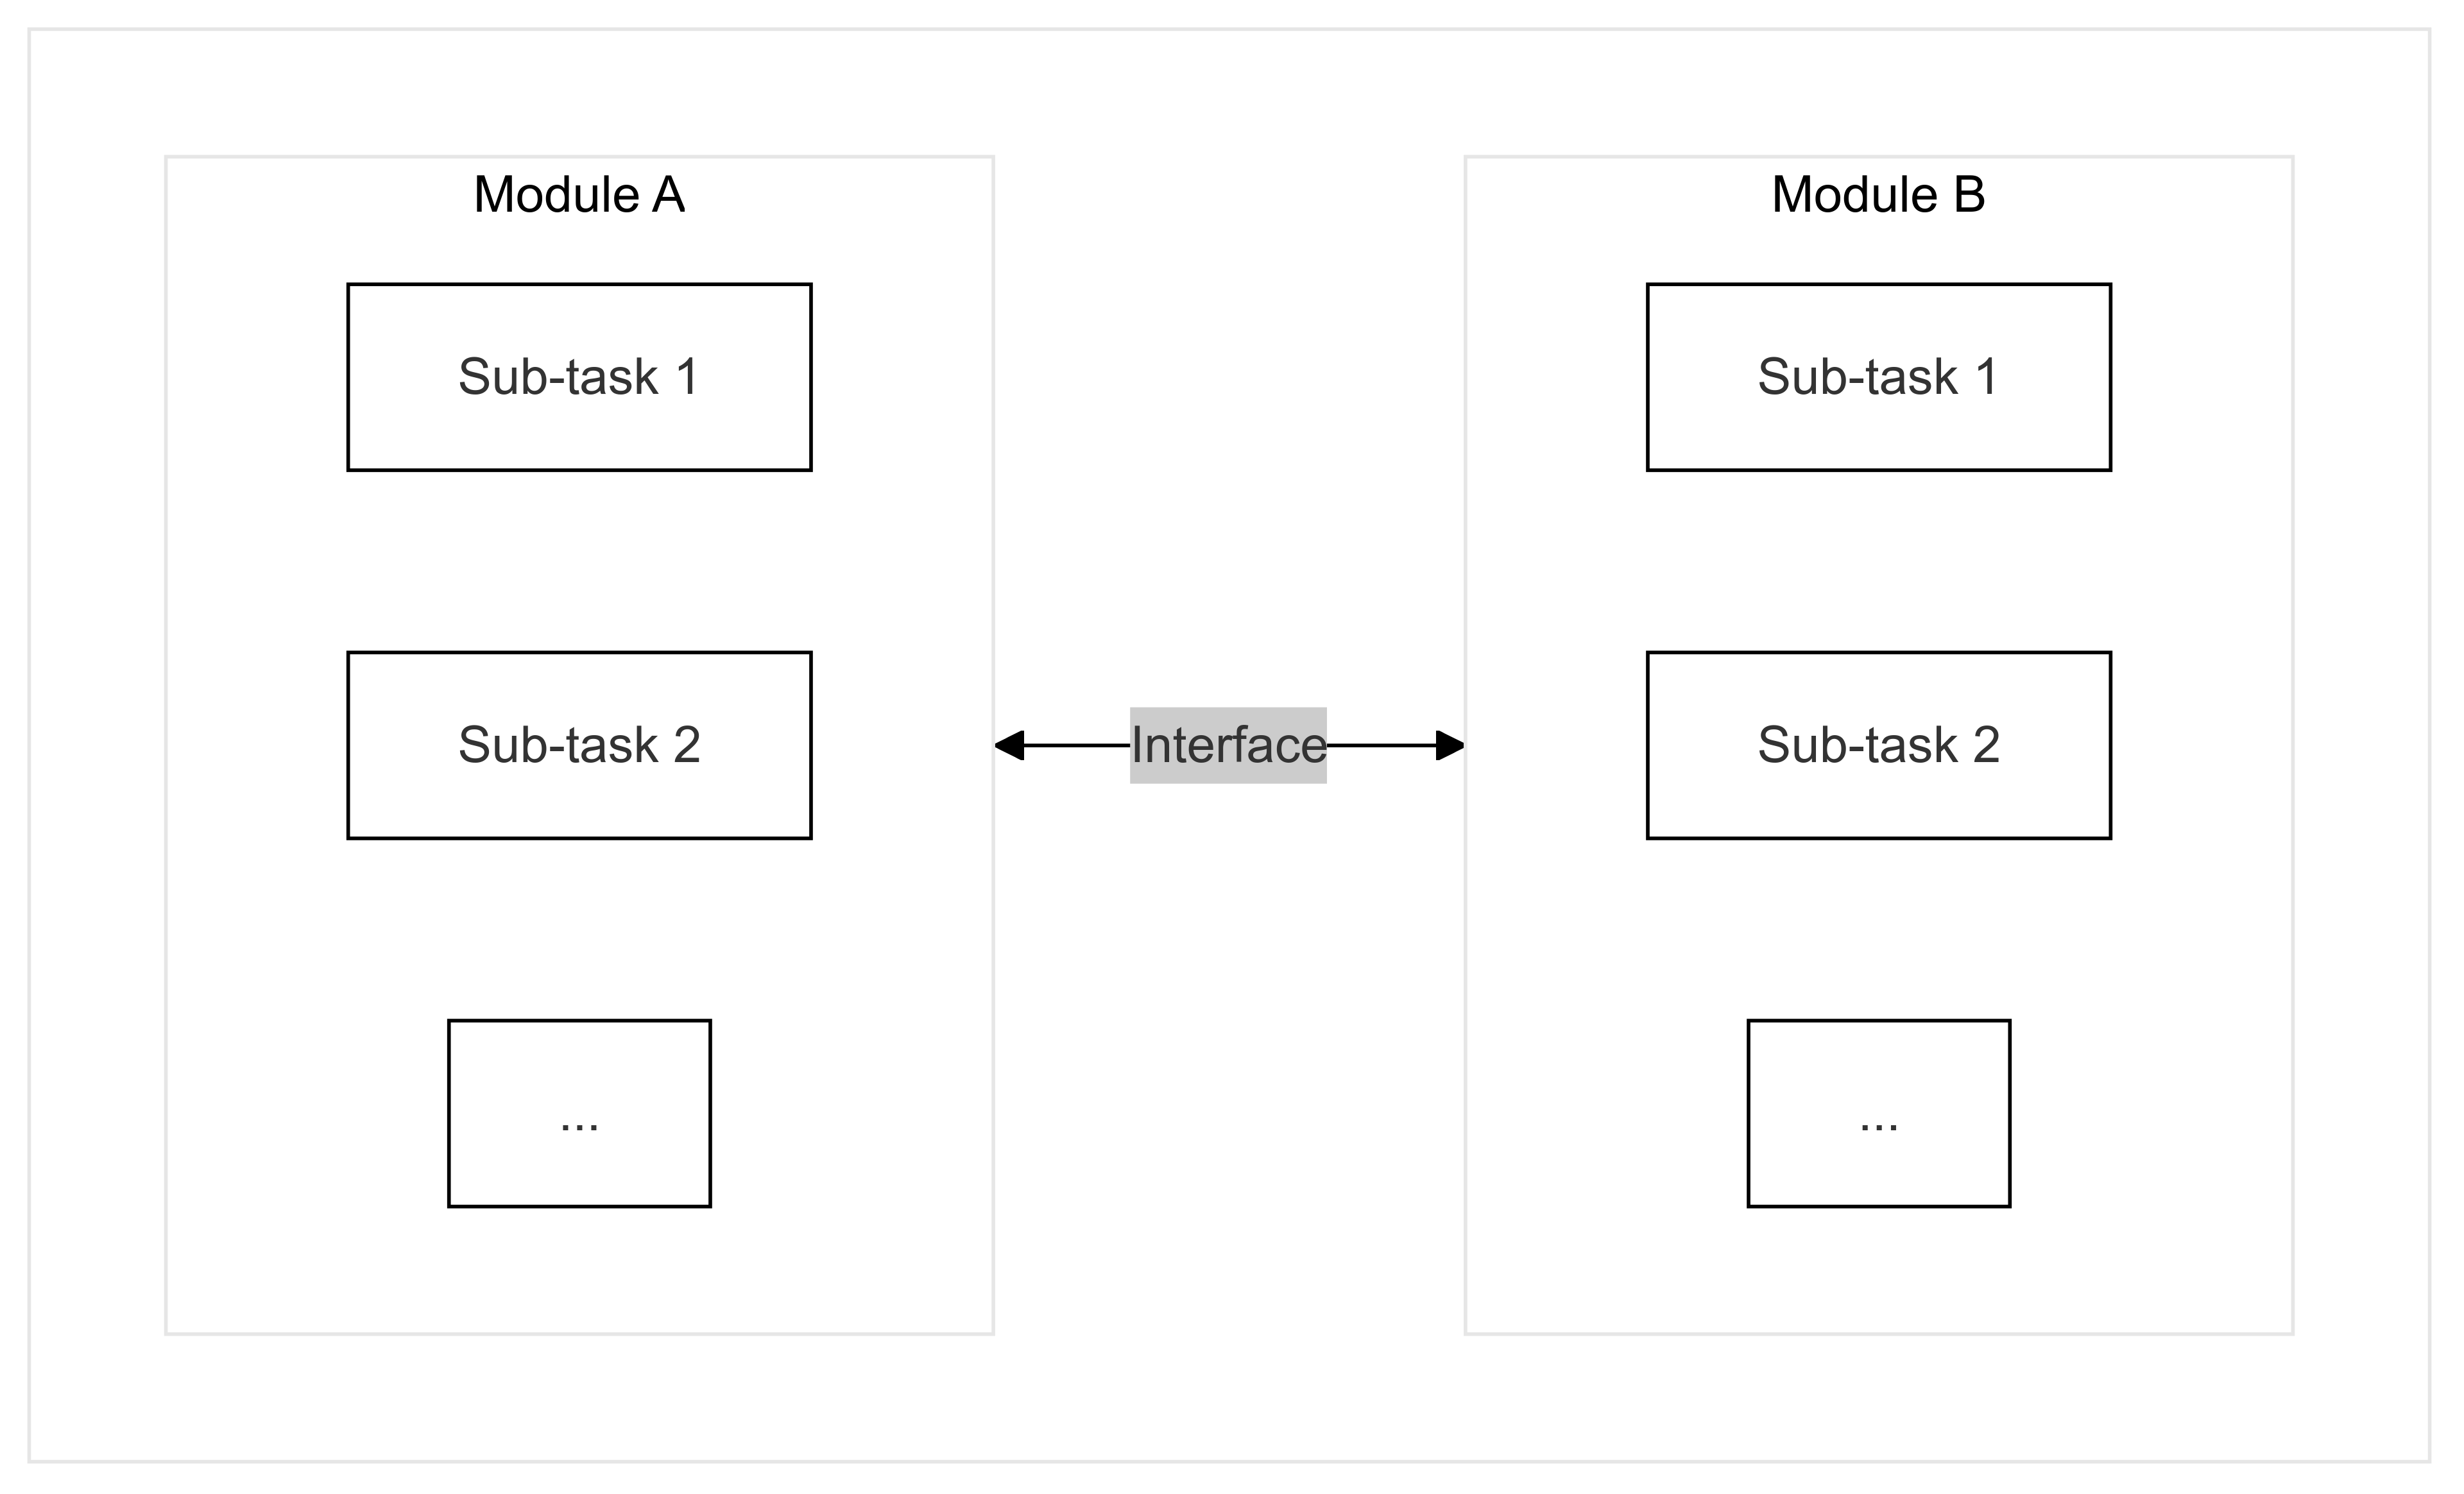
\includegraphics[width=0.7\textwidth]{modularity/horizontal.png}
%     \caption{Horizontal partitioning}
%     \label{fig:mod_hor}
% \end{figure}

% \begin{figure}[hbt!]
%     \centering
%     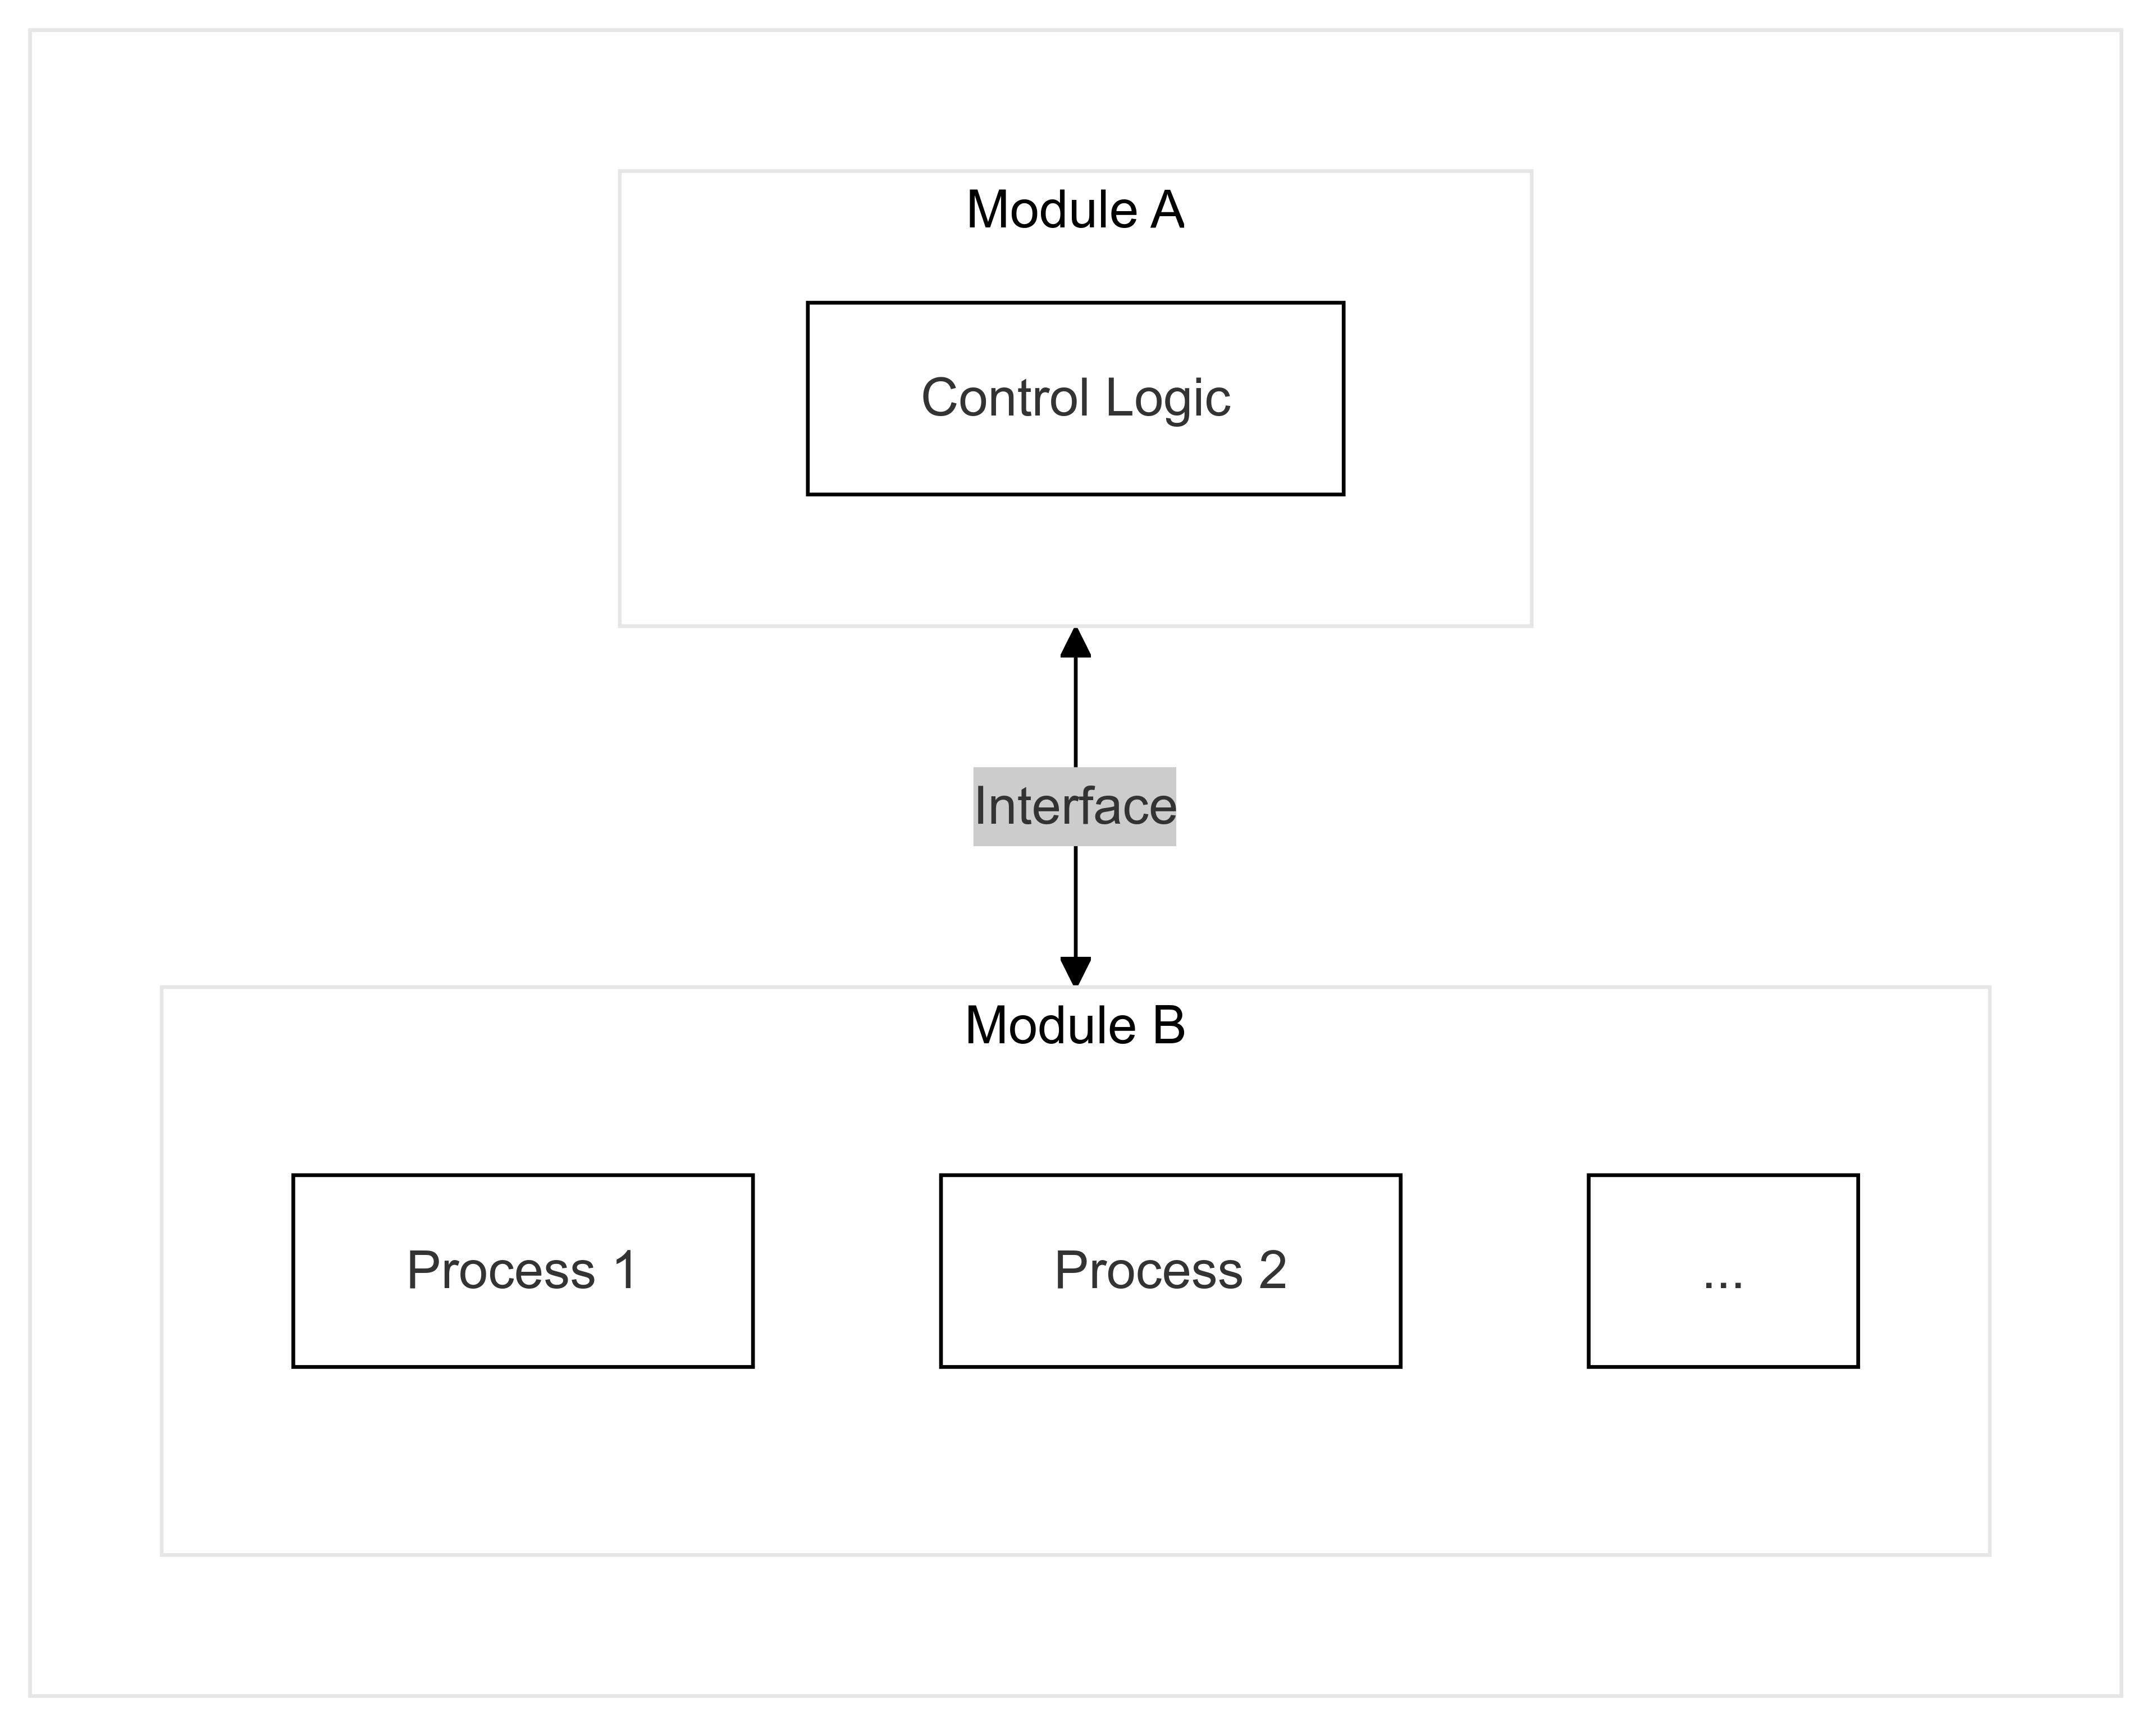
\includegraphics[width=0.7\textwidth]{modularity/vertical.png}
%     \caption{Vertical partitioning}
%     \label{fig:mod_ver}
% \end{figure}

Benefit of partitioning is the ability of software to isolate errors. Provided the software is correctly structured, an error occurring in a single module should not propagate to other modules. Meaning we can use modularity as a way to pinpoint the erroneous parts of software and attempt recovery. If recovery is not possible, the software should still be able to partially function, given that other parts of the software are not influenced by the fault. In most situations, partial functioning of a software is preferable to a complete shutdown.

\subsubsection{Error detection}

Fault-tolerant single-version application should meet two main criteria: self-protection and self-checking. Self-protection means that the application should be able to protect itself from external corruption by detecting errors in its input and output data as well as errors in its control flow. Self-checking means that the application component must be able to detect errors within itself and prevent propagation of these errors into other components \cite{nasa:sft}. These two traits combined can be together considered as the ability of "error detection".

Error detection covers a wide range of techniques used to locate errors and mitigate them. Some common approaches include:

a) checksums and \acrfullpl{ecc}, which embed additional metadata with the actual data in order to verify integrity and attempt to correct corrupted data. This approach allows for some degree of memory corruption mitigation but comes at the cost of memory overhead and additional processing per data-chunk which uses checksum or \acrshortpl{ecc}.

b) assertion and runtime checks, which perform independent checks on the data during execution which ensures the data matches the expected outcomes at certain checkpoints.

c) watchdog timers, whose main purpose is to catch deadlock states by giving a task a certain amount of time to execute before aborting it.

Error detection is a crucial aspect of single-version application, since there is no alternate version to fall back upon.

\subsubsection{Fault recovery}

Fault recovery is a process of restoring the program to a functional state after an error has been detected. Fault recovery in single-version techniques mostly consists of a program rollback, also known as \textit{backward recovery} \cite{shubu}. This can be either a full restart, effectively rolling back the program to its initial state, or a more advanced technique such as checkpoint and restart\cite{nasa:sft}.

Checkpoint and restart could be considered the basis of some of the more advanced fault tolerance techniques. Before the execution of a critical process a checkpoint is created, which captures some or all of the program state. At the end of the execution, an acceptance check is performed on the process output, if an error is detected rollback is initiated and the process is restarted.

\begin{figure}[hbt]
    \centering
    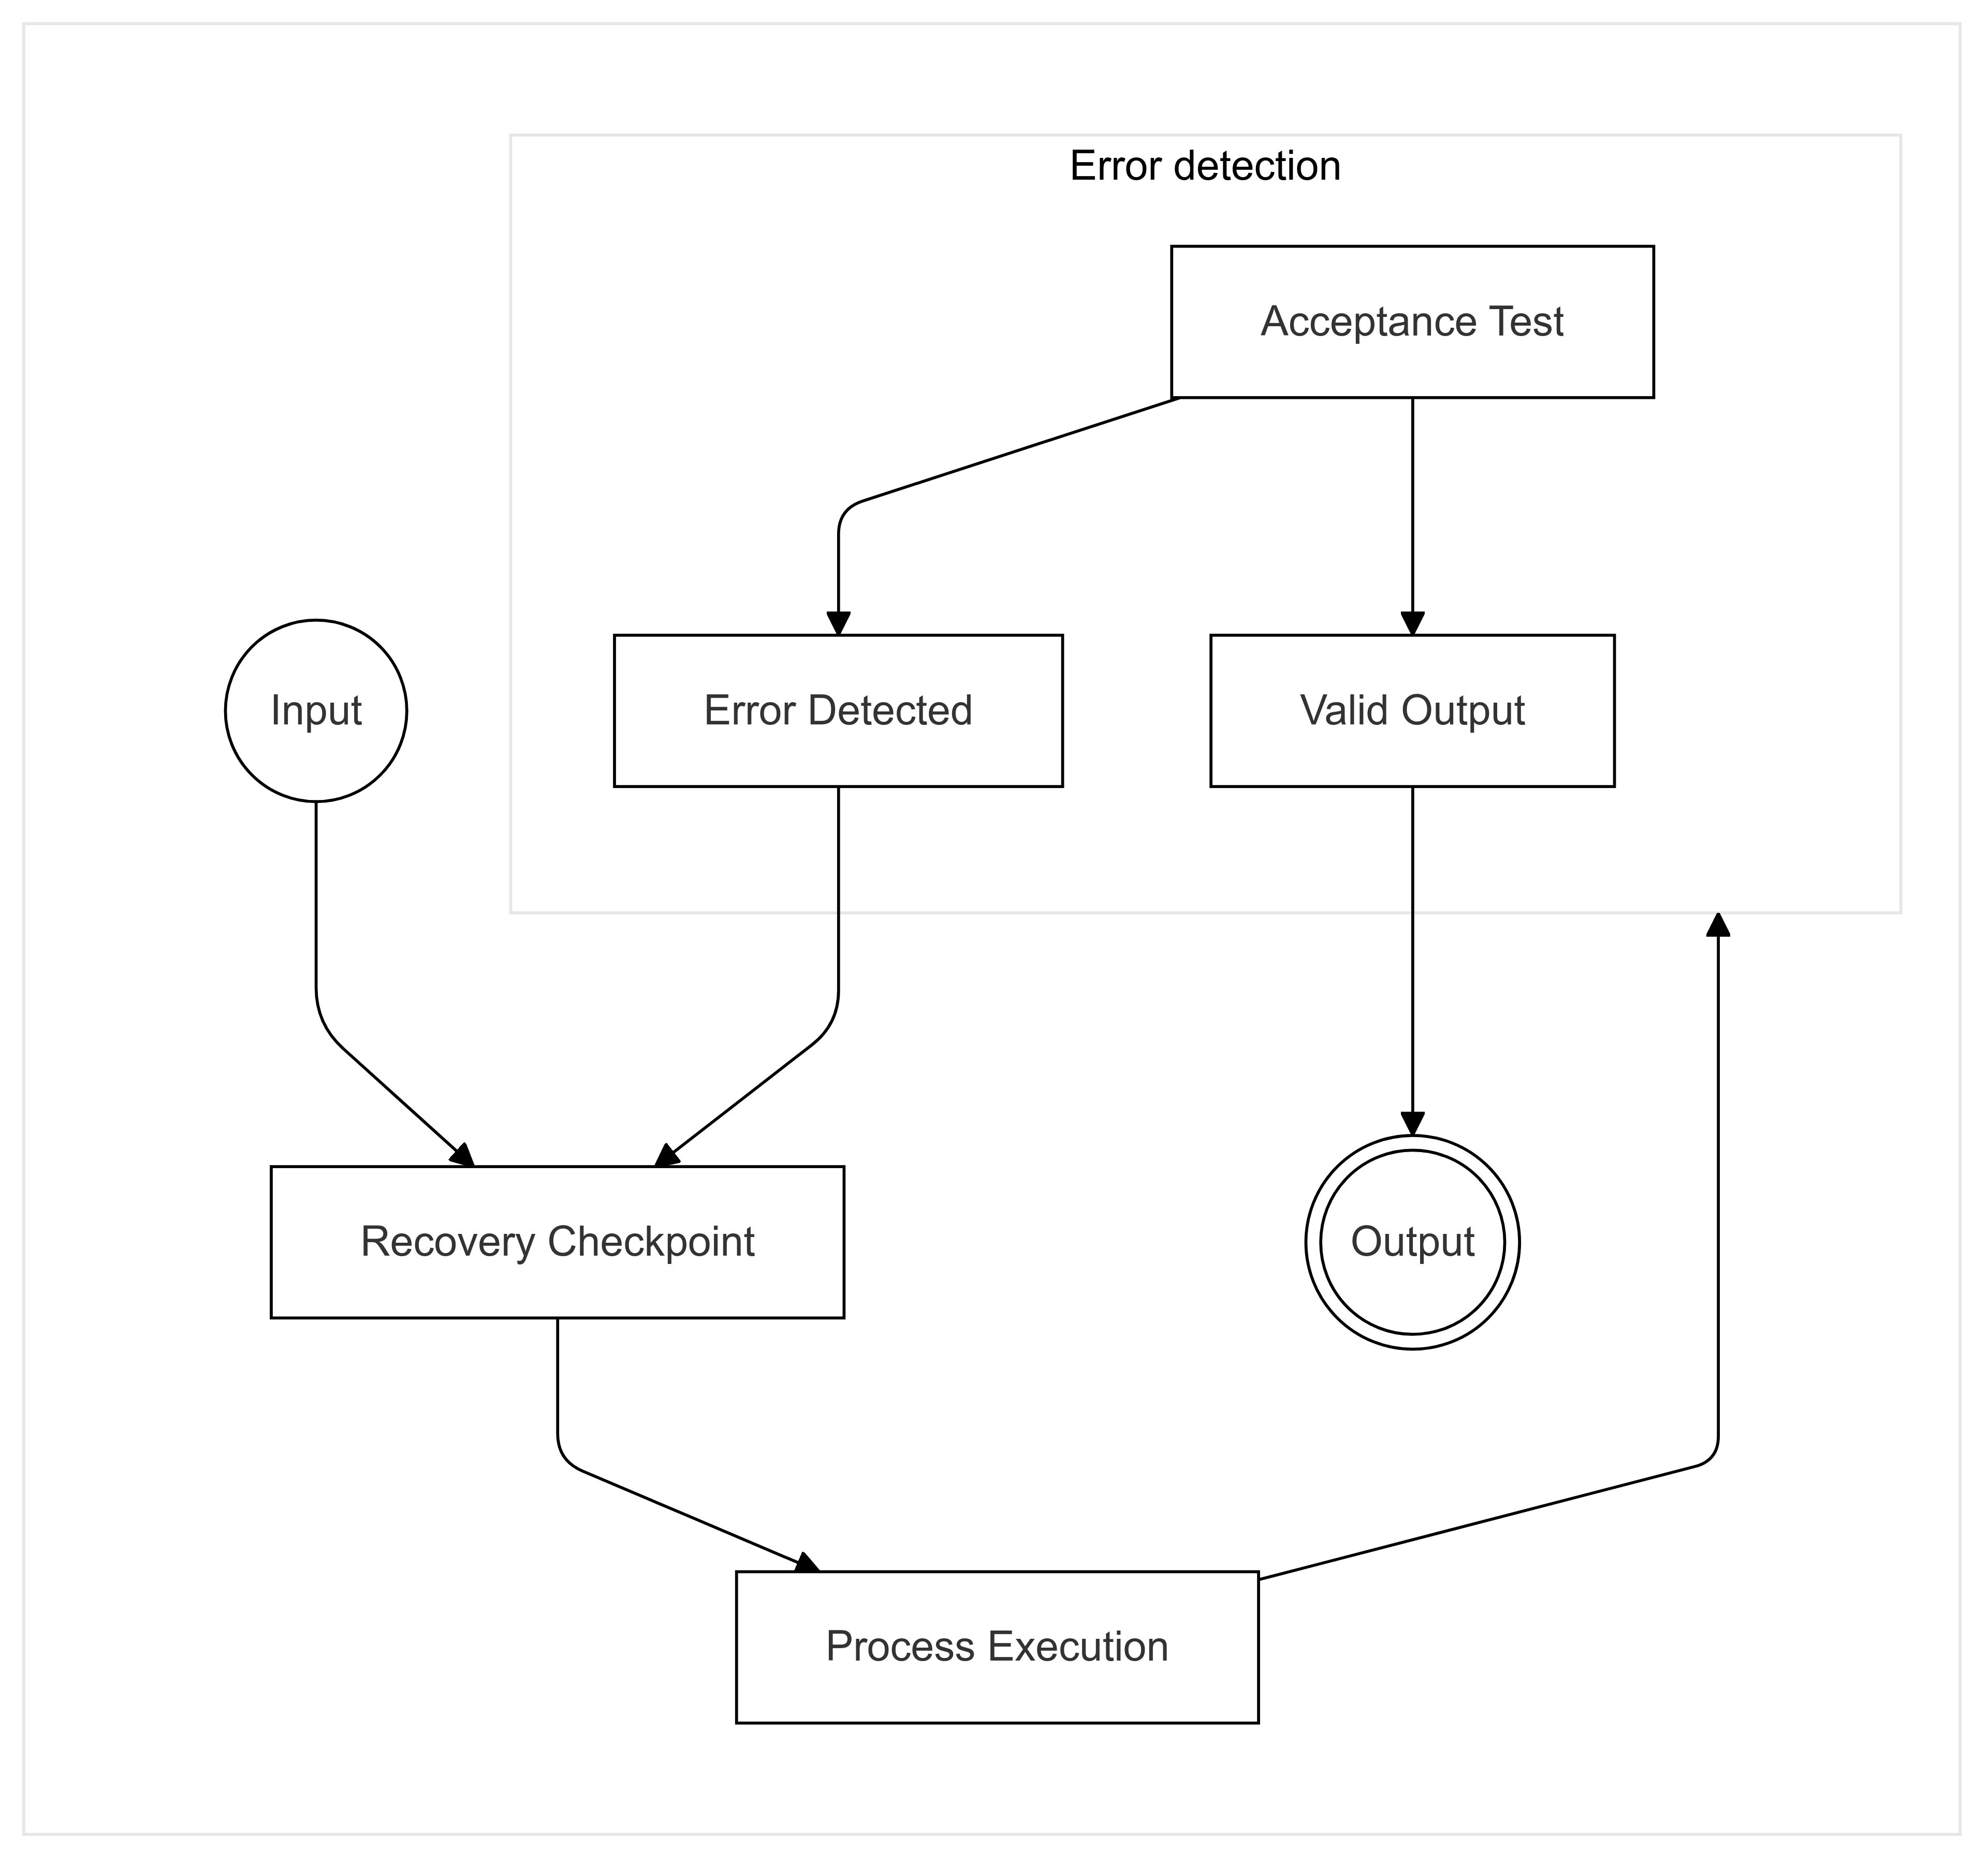
\includegraphics[width=0.7\textwidth]{diagrams/checkpoint/checkpoint.png}
    \caption{Checkpoint and restart}
    \label{fig:checkpoint}
\end{figure}

An alternative to backward recovery is \textit{forward recovery} \cite{shubu}, which is the process of correctly proceeding with execution even if error is detected. This is usually done by creating and storing three (or more copies) of critical data (\textit{data triplication}), performing the same operation on all copies, and using a majority voter to detect errors.

Forward recovery via data triplication is, generally speaking, more computationally demaning than backward recovery, since the same operation(s) has to be performed per each data copy, even during fault-free operation, and the copies have to be compared at certain synchronization points. On the other hand, backward recovery incurs minimal overhead while setting up a checkpoint and only requires additional computation when an error is actually detected.

\subsubsection{Considerations for single-version techniques}

Single-version fault tolerance techniques are largely easier to develop when compared to the ones discussed in the following section. With this relative simplicity comes the drawback of not being well suited for some situations. While these techniques should work well for transient faults that are unlikely to reoccur, a single version fault-tolerant system will fail when attempting to deal with persistent faults. Even if an error is successfully detected, single version techniques provide no clear way of dealing with errors that stem from, or are heavily influenced by the design of the system. As an example, if the memory region containing a critical function has been permanently damaged, it matters not how many times we attempt to rerun the function, it will always cause an error. For this reason, single version techniques should be reserved for parts of software which are not mission critical.

In order to effectively deal with permanent faults, we need to consider multi-version techniques covered in the following section. A lot of these techniques take inspiration from single version techniques, or even directly build on top of them.